In questo capitolo parleremo in maniera approfondita delle prove sperimentali che abbiamo effettuato sul Vadalog Resoner. \newline
Il capitolo è organizzato come segue. Nella sezione 4.1 descriveremo il tool, che ho implementato durante il mio periodo di Tesi, \emph{iWarded}, che permette la generazione di benchmark Vadalog, vedendone le funzionalità e l'implementazione. \newline
Infine nella sezione 4.2 descriveremo diversi scenari applicativi utilizzando benchmark generati con tool (ad esempio iWarded), generandone anche i dati, per testare situazioni ben precise, ad esempio la presenza di ricorsione, di propagazione dei nulli, di join tra variabili harmful, ecc.

\section{L'implementazione di iWarded}

In questa sezione descriveremo il tool \emph{iWarded}, che permette la generazione di benchmark con determinate caratteristiche che vengono espresse attraverso l'input. Inoltre gli input vengono presi di default da file csv generato e popolato dallo stesso iWarded. \newline
iWarded è stato implementato separatamente rispetto al core logico del Vadalog Reasoner e prende in input i seguenti parametri: 
\begin{itemize}
	\item Numero di regole che devono essere presenti nel programma finale.
	\item Numero medio di atomi nel corpo delle regole.
	\item Numero medio di variabili in una regola.
	\item Probabilità di avere una costante.
	\item Numero medio di join in una regola.
	\item Numero di tuple nei file di input. 
	\item Path di destinazione per il salvataggio dei file CSV e del programma.
\end{itemize}
Attraverso questi parametri presi come input, vengono svolti dei passaggi per la creazione del programma Vadalog. \newline
Si parte dal numero di regole, queste bisogna suddividerle in regole di input, intermedie e output, definendo un numero preciso. In particolare il numero di regole di input è definito nel range [1, n.regole totali/2], quindi ho almeno 1 regola di input ed al massimo la metà delle regole totali di input; stesso ragionamento per le regole di output definite nel range [1, n.regole totali/3]; ed infine il numero di regole intermedie definite come la sottrazione tra le regole totali con quelle di input ed output. \newline
Successivamente si passa alla creazione delle regole, per quelle di input è presente un modulo che si occupa:
\begin{itemize}
	\item Creazione e popolazione del file CSV nel path definito.
	\item Creazione delle regole di input (annotazioni di input e di bind).
	\item Salvataggio in cache delle regole create, che solitamente hanno un nome convenzionale che va da in\_1 ad in\_n.
\end{itemize}
Poi vengono create le regole intermedie con l'esecuzione dei seguenti passaggi:
\begin{itemize}
	\item Creazione del corpo della regola utilizzando gli atomi di input o eventuali atomi intermedi già creati, utilizzando il numero medio di atomi e variabili nel corpo e facendo join sulla base del numero medio di join.
	\item Creazione dell'atomo di testa, utilizzando un nome convenzionale che va da intermediate\_1 ad intermediate\_n.
	\item Assegnazione delle variabili in testa casuali e aggiungendo delle variabili esistenziali con una probabilità del 20\%.
	\item Infine vengono salvate in cache per essere utilizzate come corpo di altre regole intermedie o di output.
\end{itemize}
Vengono poi create le regole di output:
\begin{itemize}
	\item Viene creato il corpo utilizzando atomi sia di input che intermedi.
	\item Viene creata la testa proiettando variabili casuali dal corpo della regola, evitando variabili dangerous che potrebbero portare ad un programma non warded.
\end{itemize}
Infine l'intero modello contenente le regole create viene salvato su disco. \newline
Nell'esempio~\ref{ex26} possiamo vedere un programma generato da iWarded:
\begin{example}\label{ex26}
	\scriptsize \begin{lstlisting}
	
	@output("ou_1").
	@input("in_1").
	@bind("in_1","csv","/Users/utente/Desktop","in_1_csv.csv").
	@input("in_2").
	@bind("in_2","csv","/Users/utente/Desktop","in_2_csv.csv").
	intermediate_1(HARMLESS_1) :- in_1(HARMLESS_1,HARMLESS_2).
	intermediate_2(HARMLESS_3) :- in_2(2,HARMLESS_3).
	intermediate_3(DANGEROUS_1) :- in_1(HARMLESS_1,HARMLESS_2).
	intermediate_4(HARMLESS_1) :- in_1(HARMLESS_1,HARMLESS_2).
	ou_1(HARMLESS_4) :- intermediate_1(HARMLESS_4).
	\end{lstlisting}
\end{example}
Possiamo vedere la presenza di costanti e variabili dangerous, ma in questo caso non sono presenti join. 

\section{Scenari utilizzati}

In questa sezione descriveremo l'applicazione del Vadalog Reasoner in diversi scenari.\newline
Per effettuare i test il Reasoner è stato utilizzato come una libreria, come storage abbiamo utilizzato file CSV. \newline
La configurazione hardware per l'esecuzione dei test è la seguente:
\begin{itemize}
	\item Sistema operativo: Linux.
	\item Processore: Intel Xeon v3 con 8 cores, frequenza a 2.4GHz.
	\item RAM: 16GB.
\end{itemize}
Nella sezione 4.2.1 descriveremo il comportamento del Vadalog Reasoner utilizzando degli scenari generati da \emph{iWarded}. \newline
Nella sezione 4.2.2 utilizzeremo degli scenari generati da un altro tool simile, chiamato \emph{iBench}, descrivendo il comportamento del Vadalog Reasoner rispetto ai suoi competitor. \newline

\subsection{iWarded}

Per questo scenario abbiamo utilizzato \emph{iWarded} descritto nella sezione 4.1, che permette di generare programmi Vadalog (e quindi Warded Datalog$^\pm$) con regole lineari e non lineari, con presenza di harmful o harmless join, ricorsione, ecc. \newline
\begin{figure}[h]
	\centering
	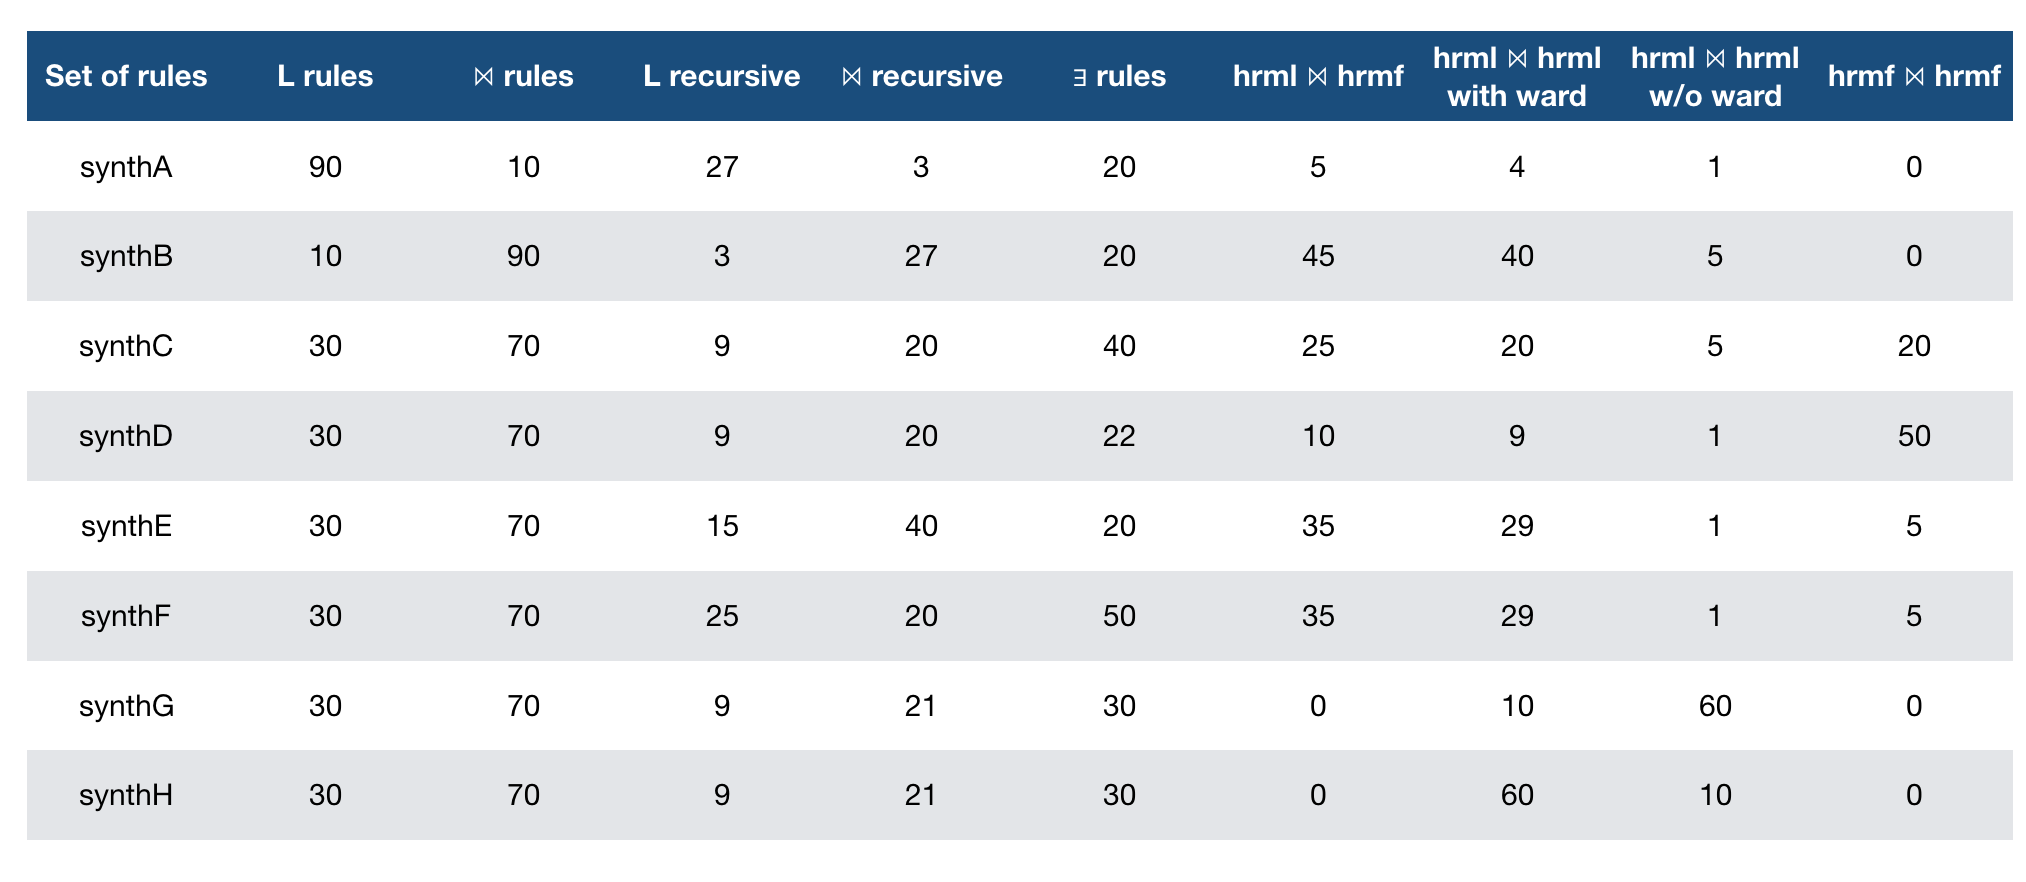
\includegraphics[width=0.8\linewidth]{figure/iWardedScenario}
	\caption{Dettagli dello scenario generato con iWarded.}
	\label{fig:iwarded}
\end{figure}

In Figura~\ref{fig:iwarded} sono rappresentati i dettagli dello scenario, in particolare per ogni set di regole (programma), abbiamo configurato delle caratteristiche:
\begin{itemize}
	\item L rules: è il numero di regole lineari presenti nel programma (regole che hanno un solo atomo nel corpo).
	\item $\bowtie$ rules: è il numero totale di regole con un join del programma.
	\item L recursive: è il numero di regole lineari ricorsive (sottoinsieme di L).
	\item $\bowtie$ recursive: è il numero di regole join ricorsive (sottoinsieme di $\bowtie$ rules).
	\item $\exists$ rules: è il numero di regole (tra lineari e $\bowtie$ rules) che hanno esattamente una variabile classificata esistenzialmente.
	\item hrml $\bowtie$ hrmf: è il numero di join tra variabili harmless e variabili harmful nell'intero programma.
	\item hrml $\bowtie$ hrml with ward: è il numero di join tra variabili harmless-harmless in regole in cui c'è una propagazione di una dangerous nella testa.
	\item hrml $\bowtie$ hrml w/o ward: è il numero di join harmless-harmless in cui non c'è la propagazione di alcuna dangerous nella testa.
	\item hrmf $\bowtie$ hrmf: è il numero di join harmful-harmful.
\end{itemize}
Abbiamo creato 8 programmi contenenti 100 regole. \newline
\emph{SynthA} ha una netta superiorità di regole lineari, il 20\% delle regole totali ha un quantificatore esistenziale, il 30\% delle regole lineari e non lineari ha una ricorsione (sia L rules che $\bowtie$ rules), ed i join sono equamente distribuiti tra harmless-harmful e harmless-harmless, quindi non sono presenti join tra valori nulli. \newline
\emph{SynthB} ha le stesse caratteristiche di SynthA, soltanto con una netta superiorità di regole non lineari (regole di join). SynthA e SynthB insieme servono a confrontare l'impatto della presenza di regole lineari. \newline
\emph{SynthC} ha tra il 30\% e il 70\% di regole lineari e non lineari, ed ha una buona presenza di join harmful-harmful sui quali ci focalizziamo. \emph{SynthD} ha lo stesso comportamento di SynthC ma ha prevalenza di join harmful-harmful. \newline
SynthC e SynthD servono a valutare l'impatto della presenza degli join harmful-harmful. \newline
\emph{SynthE} ha tutto nella media ma con una forte ricorsione sulle regole con join. \emph{SynthF} si comporta allo stesso modo di SynthE, ma ha una forte ricorsione sulle regole lineari anziché sulle regole con join. \newline
SynthE e SynthF servono a verificare l'impatto della ricorsione. \newline
\emph{SynthG} ha praticamente le stesse caratteristiche di SynthC e SynthD, ma con prevalenza di join harmless-harmless, di conseguenza ha quasi le caratteristiche di un programma Datalog. \emph{SynthH} è molto simile, ma enfatizza i join sui ward. \newline \newline
In Figura~\ref{fig:iwardedresult} sono riportati i risultati dell'esecuzione dei vari programmi. Il Vadalog Reasoner ha le migliori prestazioni sugli scenari SynthB e SynthH, con un tempo di esecuzione inferiore ai 20 secondi. \newline
In SynthB sono presenti circa 45 join harmless-harmful ma non condizionano le prestazioni del sistema. Lo scenario SynthC ha un numero medio di regole (tra lineari e non lineari) ed ha un numero bilanciato delle tipologie di join, invece SynthD ha un numero di join harmful-harmful maggiore ed impiega soltanto 7 secondi in più di SynthC, questo poiché interviene l'ottimizzazione degli harmful-harmful join trasformandoli in join harmless-harmless dove possibile (linearizzazione). Lo scenario SynthG ha 60 join harmless-harmless senza wards, è molto simile a SynthD, ma ha un tempo di reasoning maggiore dovuto alla presenza di variabili esistenziali. 
\begin{figure}[h]
	\centering
	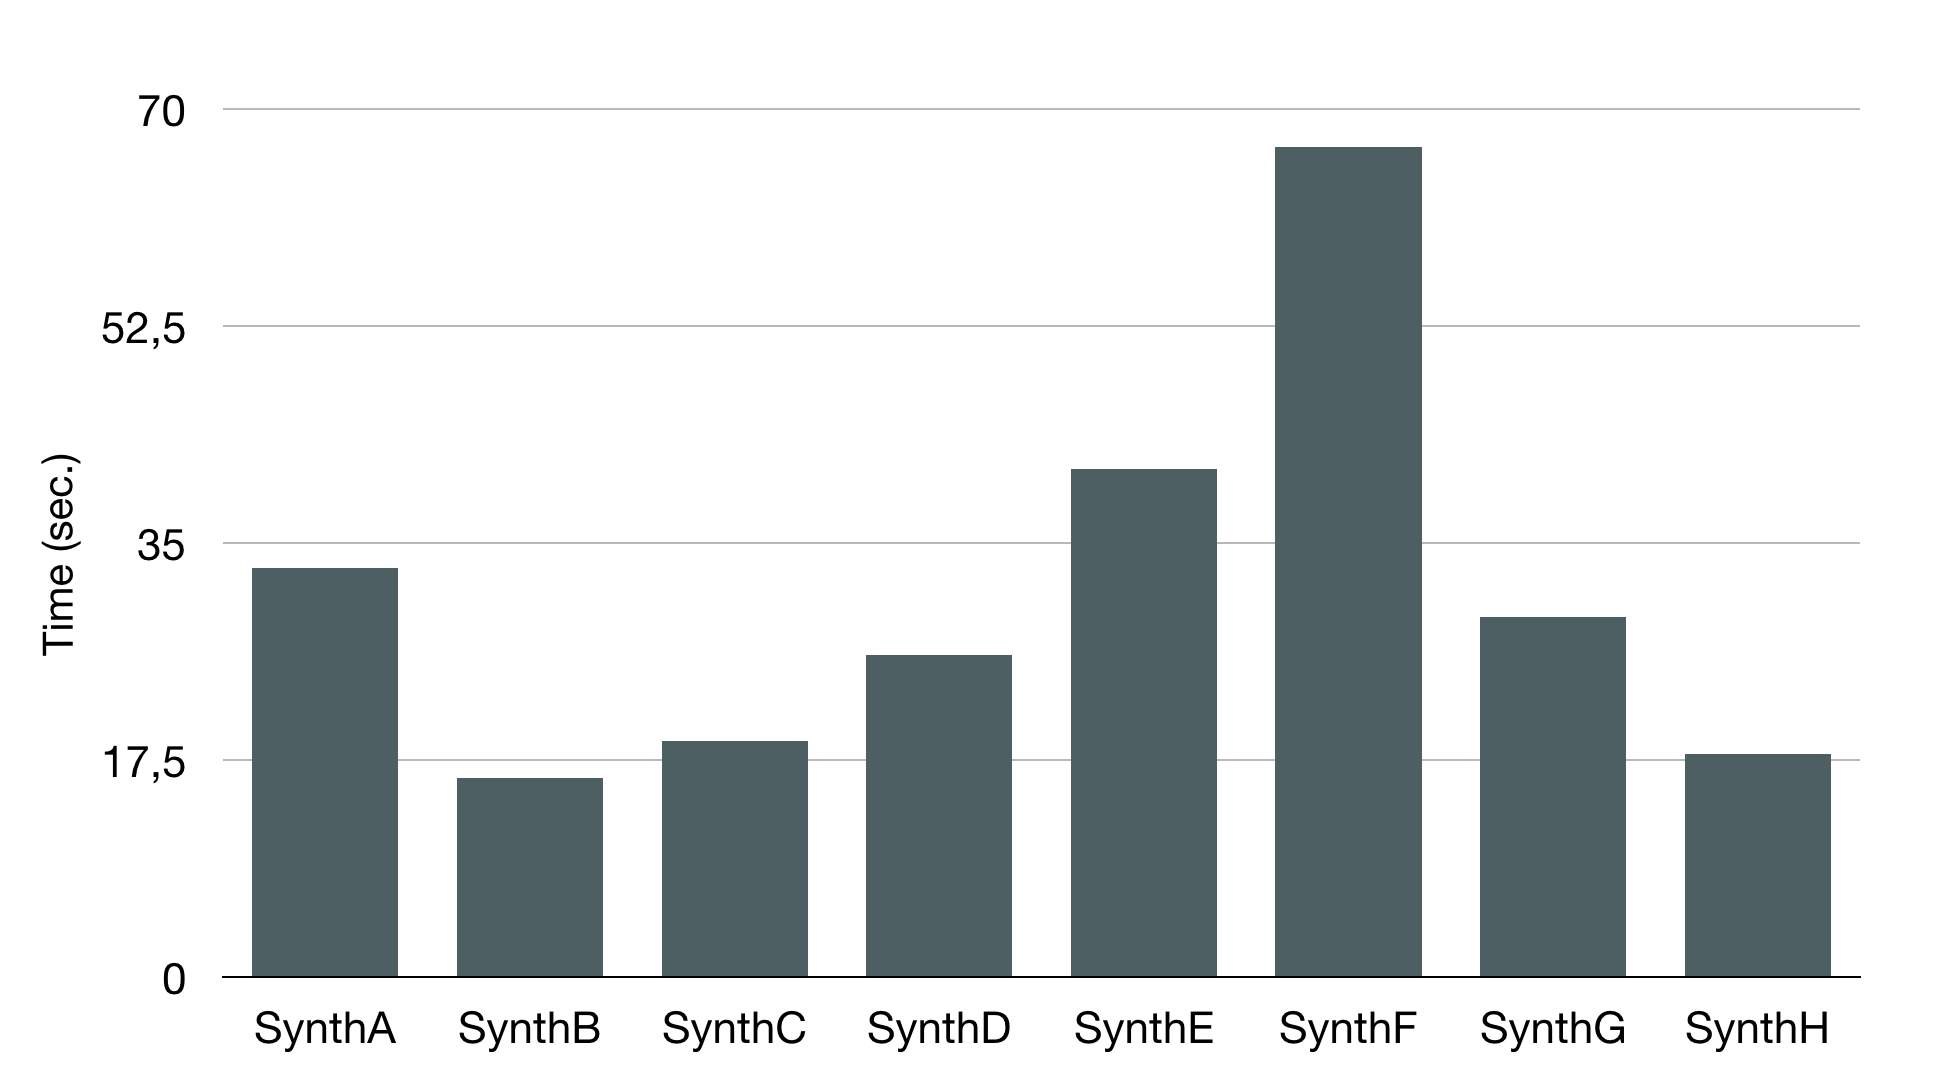
\includegraphics[width=0.8\linewidth]{figure/iWardedResult}
	\caption{Tempo di reasoning per lo scenario iWarded.}
	\label{fig:iwardedresult}
\end{figure}

Infine gli scenari SynthE e SynthF mostrano che l'impatto della ricorsione è significante, con tempi di 40 e 65 secondi rispettivamente. La ricorsione lineare ha un impatto molto forte, dovuto dalla presenza di nulli in combinazione con gli harmful join, non sfruttando a pieno i benefici dati dalla wardedness. Ciò è confermato dallo scenario SynthA, poiché ha una buona presenza di regole lineari e di ricorsione, ma non ha la presenza di join tra valori nulli, impiegando soltanto 32 secondi per l'esecuzione.

\subsection{iBench}

iBench~\cite{arocena2015ibench} è un tool per generare degli scenari di data integration. Consideriamo due famosi scenari chiamati \emph{STB-128} e \emph{ONT-256}, trasformando i programmi generati da iBench in programmi Vadalog. \newline
Questi scenari sono molto importanti per i nostri scopi, poiché hanno molte regole esistenziali, i nulli sono propagati nelle teste e coinvolti in molti join e le regole hanno una presenza molto alta di ricorsione. \newline
STB-128 è un programma che ha le seguenti caratteristiche: 
\begin{itemize}
	\item Composto da un insieme di 250 regole warded, di cui il 25\% sono esistenziali.
	\item Sono presenti 15 casi di harmful join.
	\item 30 casi di propagazione dei nulli.
	\item Ci sono 112 atomi distinti.
	\item La sorgente contiene 1000 fatti per ogni atomo.
	\item Il risultato atteso è di 800 mila fatti, di cui il 20\% nulli.
\end{itemize}
In questo scenario abbiamo eseguito 16 query differenti molto complesse, coinvolte ognuna in circa 5 join.\newline
ONT-256 è un programma che ha le seguenti caratteristiche:
\begin{itemize}
	\item Composto da un insieme di 789 regole warded, di cui il 35\% sono esistenziali. 
	\item Sono presenti 295 casi di harmful join.
	\item Più di 300 casi di propagazione dei nulli.
	\item Ci sono 220 atomi distinti.
	\item La sorgente contiene 1000 fatti per ogni atomo.
	\item Il risultato atteso è di circa 2 milioni di fatti, di cui il 50\% nulli.
\end{itemize}
In questo scenario le regole sono molto più complesse rispetto a STB-128 e contengono join multipli e ricorsione. Abbiamo eseguito 11 query differenti, coinvolte ognuna in circa 5 join. \newline
L'obiettivo di questo scenario è testare i tempi di esecuzione del Vadalog Reasoner con altri sistemi di reasoning già esistenti, in particolare abbiamo considerato i sistemi: RDFox~\cite{motik2014parallel}, Llunatic~\cite{geerts2014s}, DLV~\cite{leone2006dlv}, Graal~\cite{baget2015graal} e PDQ~\cite{benedikt2015querying}. \newline
In Figura~\ref{fig:ibenchgrafico} vengono messi a paragone i tempi di reasoning del Vadalog Reasoner e tutti gli altri sistemi menzionati utilizzando la stessa configurazione hardware/software. \newline
Come possiamo vedere dal grafico il Vadalog Reasoner ha prestazioni migliori su entrambi i scenari, con un tempo di 6.59 secondi per l'esecuzione di STB-128 e 51.579 secondi per ONT-256, ed è in media 3 volte maggiore rispetto a RDFox, 7 volte maggiore rispetto a Llunatic.\newline 
In particolare i sistemi RDFox, Llunatic e DLV hanno rispettivamente 28, 52 e 48 secondi di esecuzione per STB-128 e 83, 367, 118 secondi di esecuzione per ONT-256.
\begin{figure}[h]
	\centering
	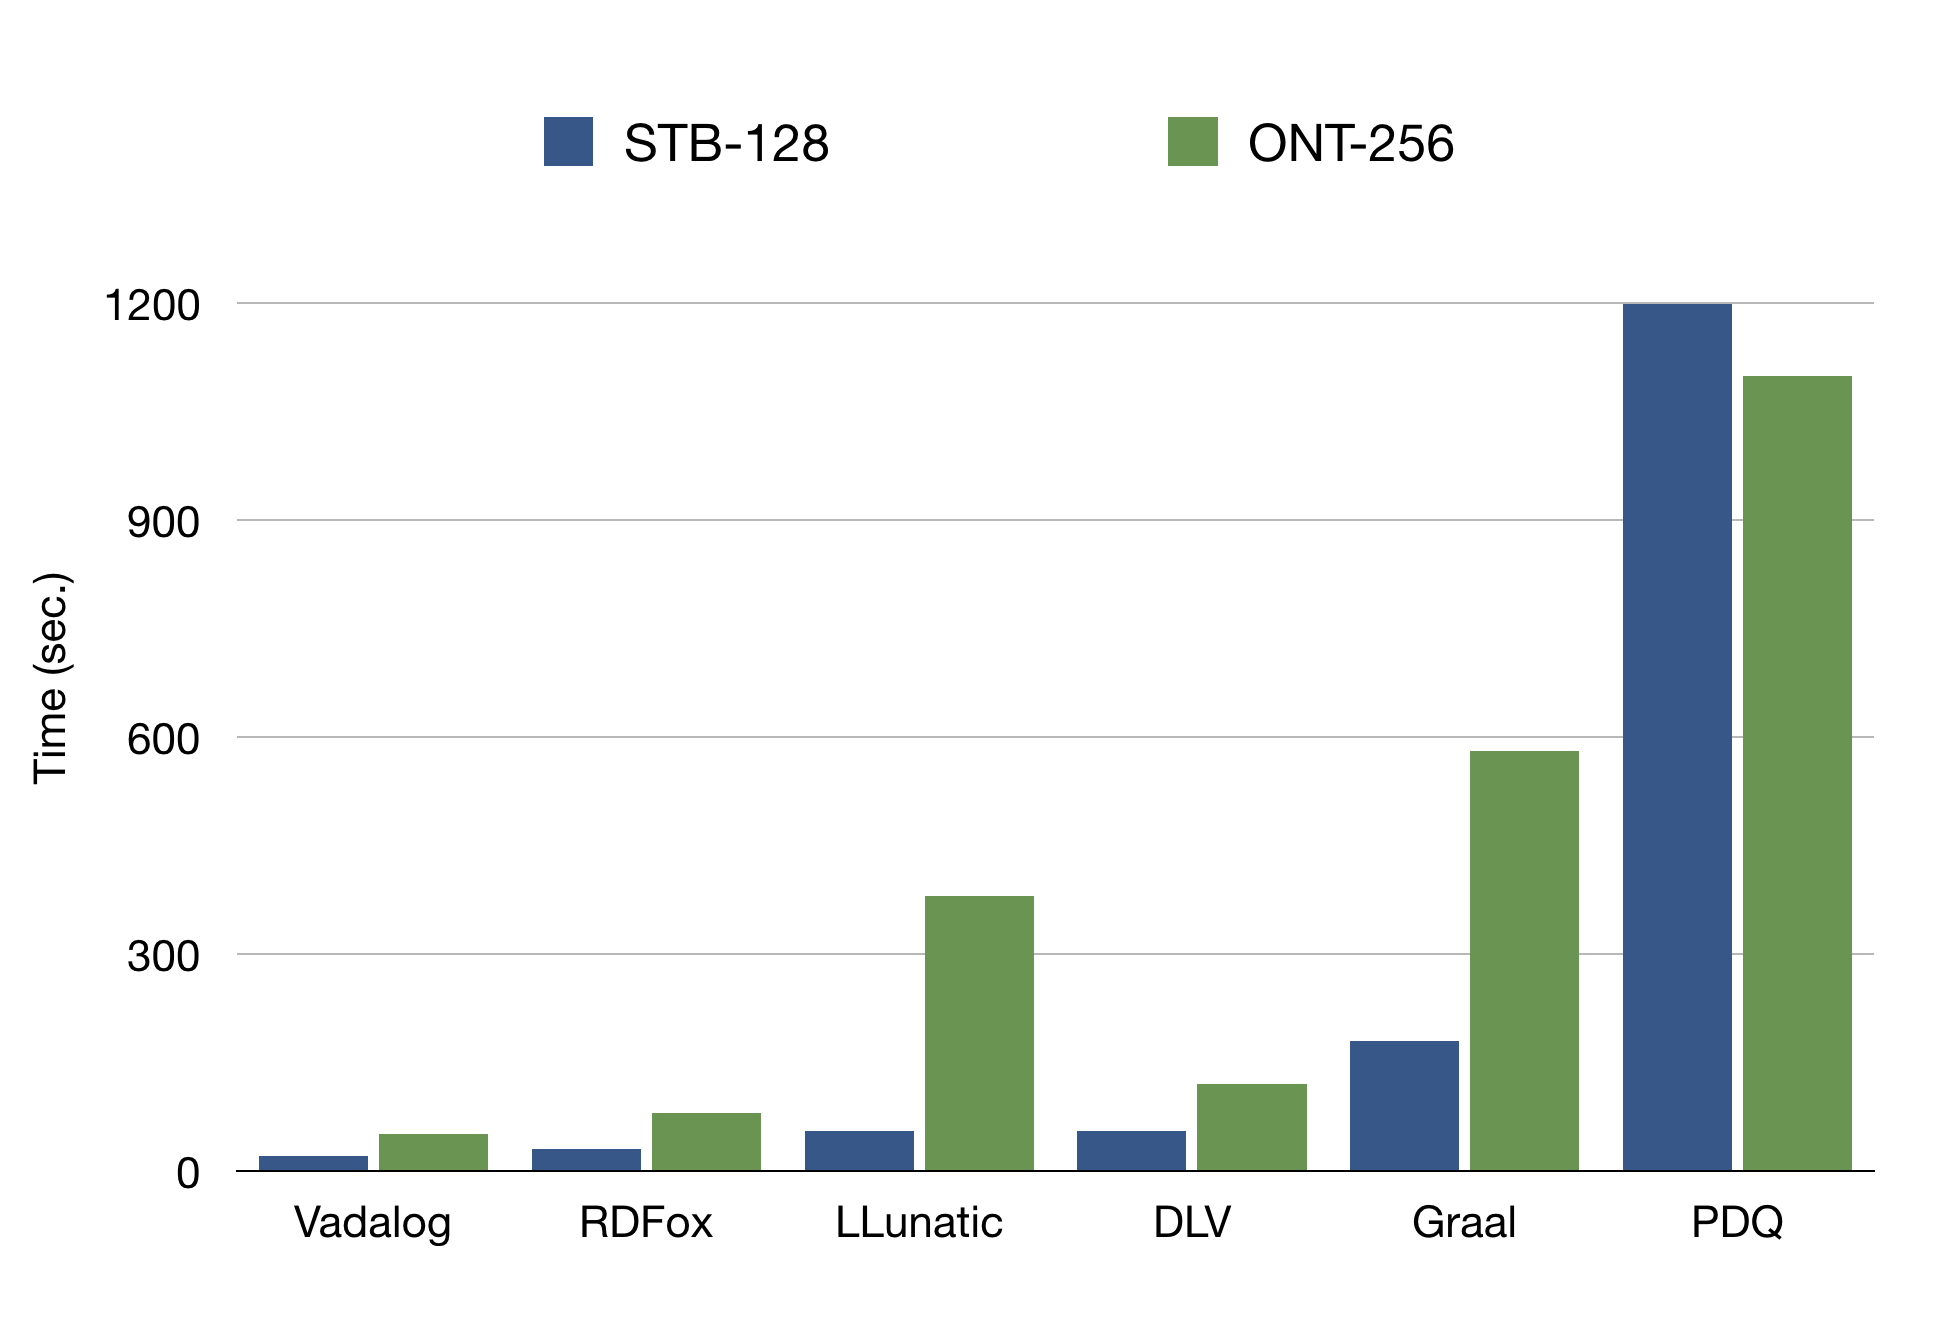
\includegraphics[width=0.8\linewidth]{figure/ibenchgrafico}
	\caption{Tempo di reasoning per gli scenari STB-128 e ONT-256 su tutte le piattaforme.}
	\label{fig:ibenchgrafico}
\end{figure}